%! Licence = CC BY-NC-SA 4.0

%! Author = gianfluetsch
%! Date = 22. Jan 2022
%! Project = icth_summary

\section{Kanalcodierung}

\subsection{Blockcode}
\subsubsection{Nachprüfung HS2020}
$x_5=x_1+x_2+x_3$\\
$x_6=x_1+x_2+x_4$\\
$x_7=x_2+x_3+x_4$

\paragraph{Prüfmatrix des Blockcodes}\mbox{}\\
$\begin{matrix}
    x_1 & x_2 & x_3 & x_4 & | & x_5 & x_6 & x_7\\
    1 & 1 & 1 & 0 & | & 1 & 0 & 0\\
    1 & 1 & 0 & 1 & | & 0 & 1 & 0\\
    0 & 1 & 1 & 1 & | & 0 & 0 & 1
\end{matrix}$

\paragraph{Anzahl Kontrollstellen}\mbox{}\\
Anzahl Kontrollstellen = Anzahl 1 in Prüfmatrix (Einheitsmatrix) $\rightarrow$ 3

\paragraph{Anzahl gültige Codeworte mit Blockcode}\mbox{}\\
gültige Codeworte = Anzahl Spalten ohne Prüfmatrix\\
$m=4 \rightarrow 2^m=2^4=16$

\paragraph{Fehlersyndom, falls x1 und x2 gestört}\mbox{}\\
$110$\\
$111$\\
$--$\\
$001$

\paragraph{Fehler erkennen}\mbox{}\\
Ja, der Fehler (Syndrom) liegt in der Spalte $x_7$ der Prüfmatrix.
Geht man nun davon aus, dass nur ein Fehler passiert ist, so wird man hier eine Falschkorrektur vornehmen
(durch flippen des siebten Bits)

\paragraph{Fehler korrigieren?}\mbox{}\\
Nein, Fehler kann nicht korrigiert werden, da er in der regulären Prüfmatrix nicht gefunden wurde.

\subsubsection{Prüfung Fs2017}
Gegeben ist die folgende Generatormatrix eines systematischen Blockcodes mit den Prüfvektoren $p_1$ bis $p_7$:
$\begin{matrix}
    p_1 & p_2 & p_3 & p_4 & p_5 & p_6 & p_7\\
    1 & 0 & 1 & 1 & 0 & 0 & 0\\
    1 & 1 & 1 & 0 & 1 & 0 & 0\\
    1 & 1 & 0 & 0 & 0 & 1 & 0\\
    0 & 1 & 1 & 0 & 0 & 0 & 1
\end{matrix}$

\paragraph{Wie viele Nachrichtenstellen m hat der Code?}\mbox{}\\
Code hat 3 Nachrichtenstellen

\paragraph{Wie viele Kontrollstellen k hat der Code?}\mbox{}\\
Der Code hat 4 Kontrollstellen

\paragraph{Wie lautet das Fehlersyndrom, wenn nur das dritte Bit einer Nachricht falsch übertragen wird?}\mbox{}\\
101

\paragraph{Ermitteln Sie die Hamming-Distanz des Codes}\mbox{}\\
$H=4$\\
Es müssen mindestens 4 Prüfvektoren addiert werden, um den Orginalen-Vektor zu erhalten.

\paragraph{Ist der Code dicht gepackt?}\mbox{}\\
Der Code ist nicht dichtgepackt, da $H=4$ ist. Damit liegt mindestens 1 Codewort (CW) ausserhalb \textit{einer Korrigierkugel}.


\subsection{Zyklischer Code}
\subsubsection{Nachprüfung HS2020}
Gegeben ist folgendes Generatorpolynom:
$p(x)=x^5+x^3+x^2+1$

\paragraph{Wie viele Kontrollstellen hat Code}\mbox{}\\
Grad 5 $\rightarrow$ 5 Kontrollstellen

\paragraph{Schieberegister}\mbox{}\\
\begin{center}
    \vspace{-8pt}
    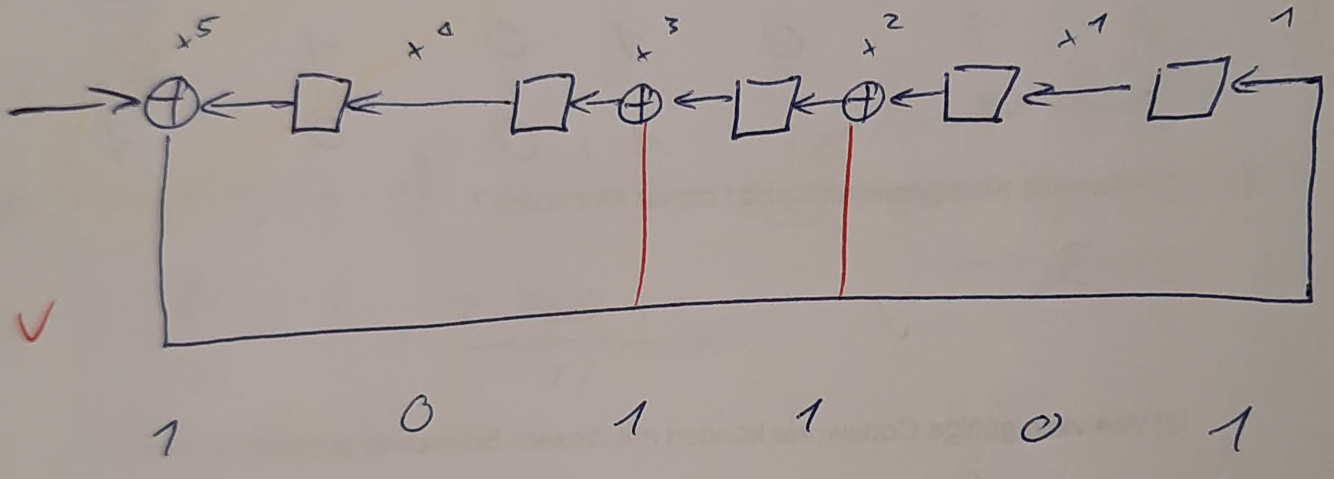
\includegraphics[width=.8\linewidth]{./02-kanalcodierung/schieberegister}
    \vspace{-8pt}
\end{center}

\paragraph{Prüfen, ob Codewort gültig}\mbox{}\\
Prüfmatrix aus Schieberegister ablesen (101101).
\begin{center}
    \vspace{-8pt}
    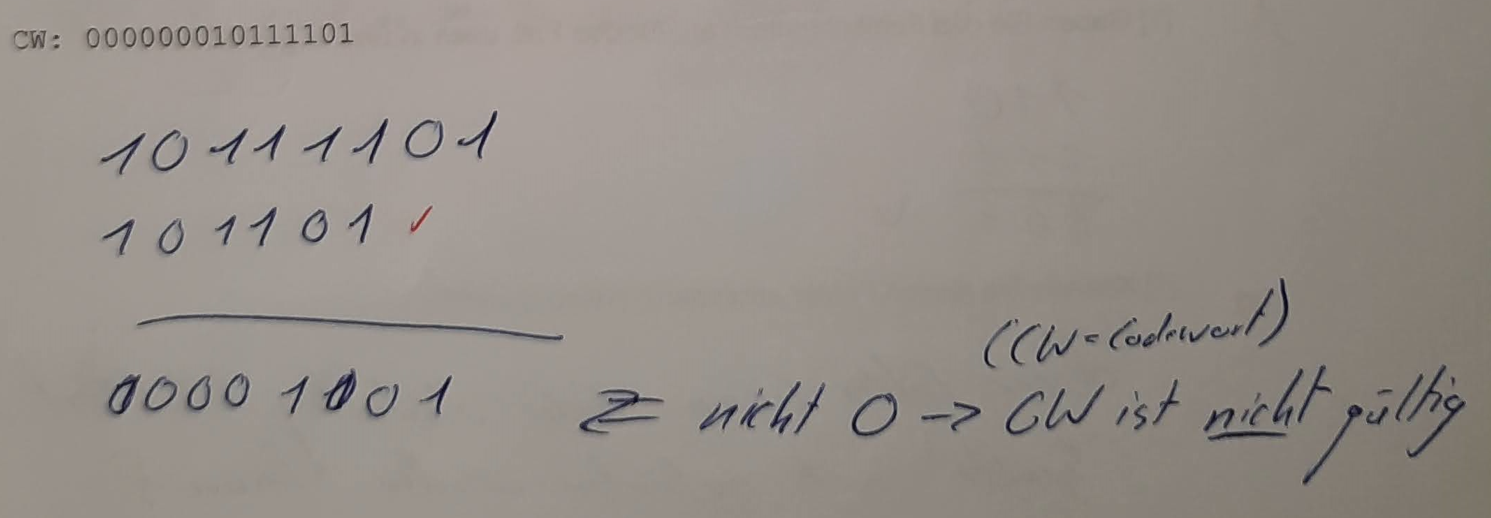
\includegraphics[width=.8\linewidth]{./02-kanalcodierung/codewort}
    \vspace{-8pt}
\end{center}

\paragraph{Fehlersyndrom für Stelle $x^5$ mit Polynomdivison ermitteln}\mbox{}\\
$x^5:x^3+x^2+1 \rightarrow Rest: x+1$

\subsubsection{Prüfung FS2017}
Gegeben ist das folgende Generatorpolynom:\\
$g(x)=x^4+x^3+x^2+1$

\paragraph{Ist das Generatorpolynom irreduzibel?}\mbox{}\\
\begin{center}
    \vspace{-8pt}
    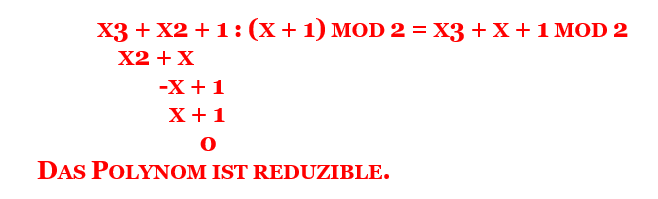
\includegraphics[width=.8\linewidth]{./02-kanalcodierung/fs2017}
    \vspace{-8pt}
\end{center}

\paragraph{Ermitteln Sie die Kontrollstellen für die Nachricht m=100}\mbox{}\\
\begin{center}
    \vspace{-8pt}
    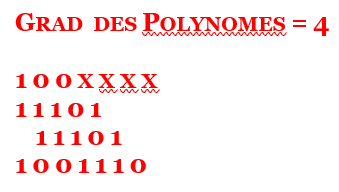
\includegraphics[width=.5\linewidth]{./02-kanalcodierung/fs2017_1}
    \vspace{-8pt}
\end{center}

\paragraph{Ermitteln Sie die Zyklusfolge des Polynoms}\mbox{}\\
$A4+A3+A2=1$\\
$0,(1=A0),A,A2,A3$\\

$A4=A3+A2+1$\\

$A5 = A4 + A3 + A = A3 + A2 + 1 +  A3 + A =  A2 + A + 1$\\
$A6= A3 + A2 + A$\\
$A7= A4 + A3 + A2 = A3 + A2 + 1 + A3 + A2 = 1$\\
Somit ergibt sich der Zyklus zu: 0001, 0010, 0100, 1000, 1101, 1110, 0001


\subsection{Faltungscode}
\subsubsection{Nachprüfung HS2020}\mbox{}\\
\begin{center}
    \vspace{-8pt}
    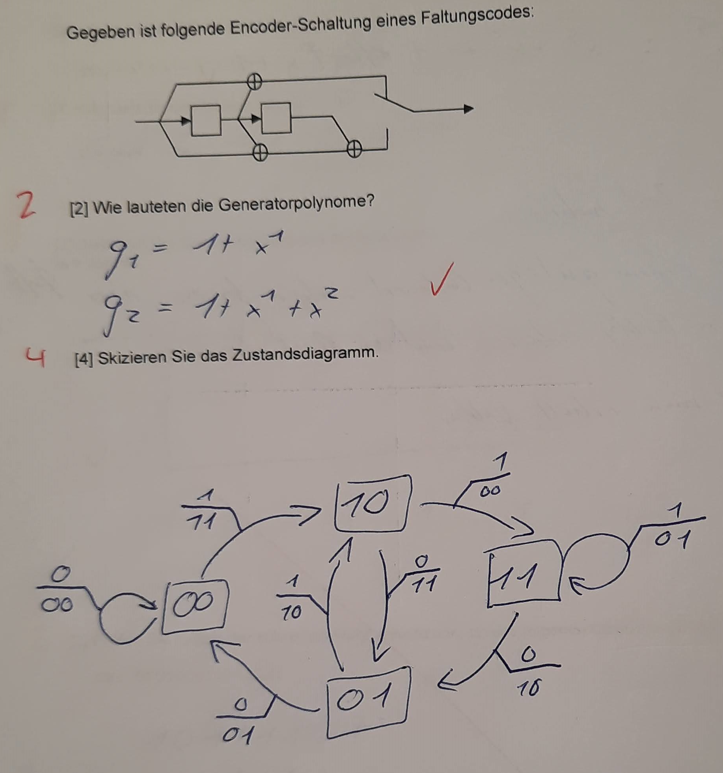
\includegraphics[width=.8\linewidth]{./02-kanalcodierung/faltungscode}
    \vspace{-8pt}
\end{center}

\subsubsection{Prüfung FS2017}
Gegeben ist der folgende Faltungscodierer
\begin{center}
    \vspace{-8pt}
    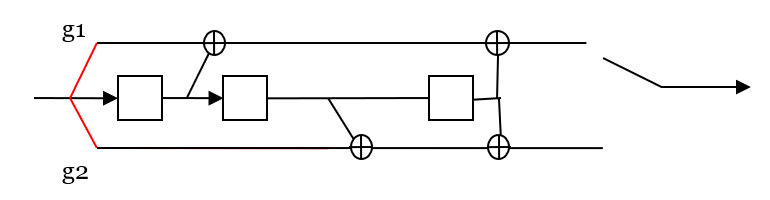
\includegraphics[width=.8\linewidth]{./02-kanalcodierung/fs2017_2}
    \vspace{-8pt}
\end{center}

\paragraph{Wie viele Bits werden zur Berechnung der Ausgangsbit herangezogen?}\mbox{}\\
4, drei aus dem Speicher und das aktuelle


\paragraph{Bestimmen Sie die Impulsantwort der Decoderschaltung}\mbox{}\\
\begin{center}
    \vspace{-8pt}
    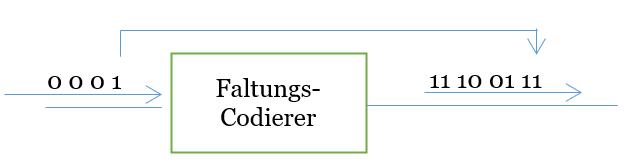
\includegraphics[width=.8\linewidth]{./02-kanalcodierung/fs2017_3}
    \vspace{-8pt}
\end{center}

\paragraph{Geben Sie die Codes in Polynomdarstellung an}\mbox{}\\
$g_1=x^3+x+1$\\
$g_2=x^3+x^2+1$

\paragraph{Wie viele Zustände hat der Coder?}\mbox{}\\
8

\paragraph{Bestimmen Sie seine Coderate}\mbox{}\\
$\frac{Anzahl Ausgangsbits}{Anzahl Eingangsbits} = \frac{8}{4}=2$\\

\subsubsection{Prüfung HS2016}
Gegeben seien die folgenden Impulsantworten eines (3,1,2)-Faltungscodierers:\\
${g_1}={1,1,0}, {g_2}={1,0,1} \& {g_3}={1,1,1}$\\

\paragraph{Zeichnen Sie die Encoder Schaltung}\mbox{}\\
\begin{center}
    \vspace{-8pt}
    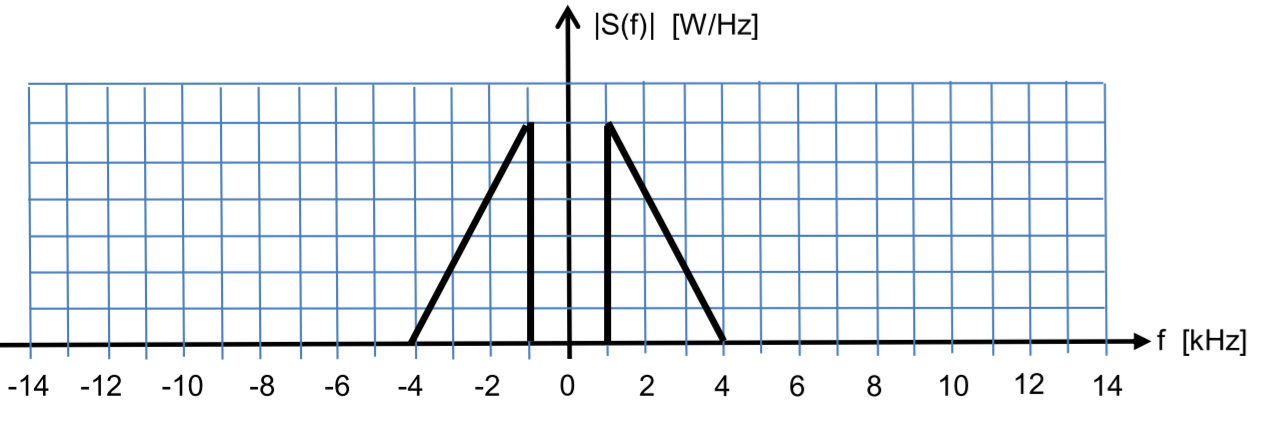
\includegraphics[width=.8\linewidth]{./02-kanalcodierung/hs2016}
    \vspace{-8pt}
\end{center}

\paragraph{Wie viele Tail-Bits müssen einer Nachrichtenfolge angefügt werden?}\mbox{}\\
2 TAIL-BITS

\paragraph{Geben Sie das Encoder-Zustandsdiagramm an}\mbox{}\\
\begin{center}
    \vspace{-8pt}
    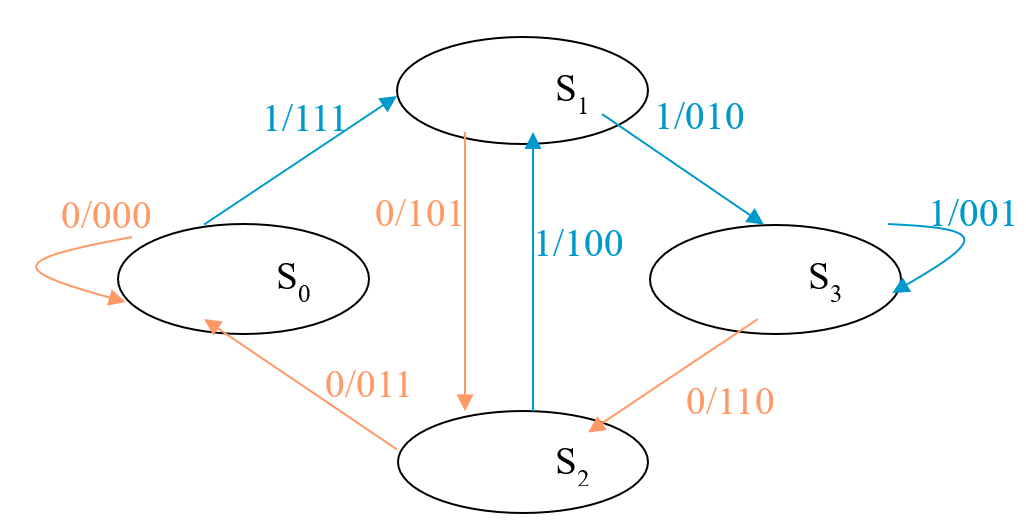
\includegraphics[width=.8\linewidth]{./02-kanalcodierung/hs2016_1}
    \vspace{-8pt}
\end{center}

\paragraph{Liegt ein katastrophaler Code vor (Begründung)?}\mbox{}\\
Nein, da es keine Zyklen ohne Gewichtszunahme gibt.

\paragraph{Bestimmen sie die (Block)-Coderate}\mbox{}\\
$B=Eingabebits$\\
$R=\frac{B}{N} = \frac{B}{3*(B+2)}$



\subsection{Kanalmatrix}
\subsubsection{Prüfung HS2016}
Die Eigenschaften eines Kanals seien durch die folgende Kanalmatrix beschrieben: 

$P(Y|X) = \begin{matrix}
    0.4 & 0.5 & 0.1\\
    0.3 & 0.4 & 0.3\\
    0.3 & 0.1 & 0.6
\end{matrix}$

\paragraph{Bestimmen Sie die Entscheidungszuordnung nach dem Maximum Likelyhood-Verfahren:}\mbox{}\\
$P(Y|X) = \begin{matrix}
    \textcolor{red}{0.4} & \textcolor{red}{0.5} & 0.1\\
    0.3 & 0.4 & 0.3\\
    0.3 & 0.1 & \textcolor{red}{0.6}
\end{matrix}$

\paragraph{}\mbox{Maximum Likelihood}\\
Berechnen Sie die Restfehlerwahrscheinlichkeit für die nach dem Maximum Li-kelyhood-Verfahren gefundene Entscheidungszuordnung\\
Gehen Sie davon aus, dass alle Eingangszeichen gleichwahrscheinlich auftreten.\\

$p(restfehler) = 1 - [1/3*(0.4+0.5+0.6)] = 0.5$\\

In einer vertieften Analyse der Eingangszeichen wurden folgende Auftrittshäufigkeiten festge-stellt:\\
$x1 = 500$\\
$x2 = 2500$\\
$x3 = 7000$\\

Lässt sich mit dieser zusätzlichen Information eine Entscheidungszuordnung finden, die besser ist als die nach dem Maximum Likelyhood-Verfahren gefunde-ne? Begründen Sie Ihren Entscheid.
$p(x1) = 0.05$\\
$p(x2) = 0.25$\\
$p(x3) = 0.70$\\


$P(Y|X) = \begin{matrix}
    \textcolor{red}{0.4} & 0.5 & 0.1\\
    0.3 & \textcolor{red}{0.4} & 0.3\\
    0.3 & 0.1 & \textcolor{red}{0.6}
\end{matrix}$

$p(rest) = 1-(0.05*0.4 + 0.25*0.4 + 0.7*0.6) = 0.46 $\\

ist kleiner als 0.5 und auch kleiner als wenn Restfehlerwahrscheinlichkeit mit der Analyse für 	die ursprünglich gewählte Konfiguration:\\
$1 - (0.05*0.4 + 0.05*0.5 + 0.7*0.6) = 0.535$
